\documentclass[10pt,a4paper]{article}
\usepackage[margin=2.0cm]{geometry}
\usepackage[T1]{fontenc}
\usepackage{lmodern}
\usepackage[british]{babel}
\usepackage{booktabs,array,graphicx,amsmath,caption,enumitem,float}
\usepackage[numbers,sort&compress]{natbib}
\setlength{\bibsep}{1pt plus 0.3ex}
\usepackage{etoolbox}\AtBeginEnvironment{thebibliography}{\scriptsize}
\usepackage[hidelinks,breaklinks]{hyperref}
\hypersetup{
  pdftitle={A Street Corner for a Dime: Placing Don Rosa's 1877 Glasgow Shoeshine Scene},
  pdfauthor={Mickaël Labarrère},
  pdfsubject={Preprint, version 1.4; text, data, tables and diagrams CC BY 4.0; source code MIT},
  pdfkeywords={Don Rosa, Glasgow, historical GIS, Ordnance Survey, street directories, comics studies, reproducible research}
}
\captionsetup{font=small,labelfont=bf}
\setlist{nosep}
\raggedbottom
\renewcommand{\topfraction}{0.9}\renewcommand{\bottomfraction}{0.9}\renewcommand{\textfraction}{0.05}\renewcommand{\floatpagefraction}{0.85}
\newcommand{\nOpenings}{62}
\newcommand{\nCornersOriented}{32}
\newcommand{\nPhysicalCorners}{24}
\newcommand{\nUniverse}{187}
\newcommand{\nCone}{45}
\newcommand{\nCtwo}{23}
\newcommand{\nCthree}{20}
\newcommand{\nAngle}{17}
\newcommand{\nCorners}{5}
\newcommand{\nCfive}{0}
\newcommand{\nCfiveWorking}{1}
\newcommand{\nModelRatio}{2}
\newcommand{\SfourD}{27.8}
\newcommand{\SfourH}{16}
\newcommand{\Sfourd}{17.0}
\newcommand{\SfourAngle}{37}
\newcommand{\SfourOpen}{JW6}
\newcommand{\DminAll}{20.0}
\newcommand{\CfiveEnvelope}{17}
\newcommand{\CfiveWorking}{20.4}
\newcommand{\nNoRatio}{20}
\newcommand{\nNoRatioCorners}{7}
\newcommand{\nNoHand}{34}
\newcommand{\nNoHandCorners}{9}
\newcommand{\nModelCorners}{1}
\newcommand{\nModelEnvelope}{20}
\newcommand{\nModelEnvelopeCorners}{7}
\newcommand{\AnnSWD}{27.3}
\newcommand{\AnnSWAngle}{35}
\newcommand{\nSfourAdmissible}{4}
\newcommand{\nBroomielawNW}{9}
\newcommand{\WidthJamaica}{22.9}
\newcommand{\WidthHoward}{11.5}
\newcommand{\RatioJH}{2.0}
\newcommand{\RatioMirror}{0.50}
\newcommand{\DPaisleyA}{83}
\newcommand{\nPlanCone}{45}
\newcommand{\nPlanAngle}{18}
\newcommand{\nPlanCorners}{5}
\newcommand{\SfourAnglePlan}{46}
\newcommand{\AnnSWAnglePlan}{30}
\newcommand{\nCfiveWorkingPlan}{2}
\newcommand{\nCfivePlan}{0}
\newcommand{\DminPlan}{18.6}
\newcommand{\CornerAngleJH}{98}
\newcommand{\nRivals}{4}

\newcommand{\degree}{$^\circ$}
\newcommand{\repourl}{\url{https://github.com/mlabarrere/a-street-corner-for-a-dime}; archived on Zenodo, concept DOI \href{https://doi.org/10.5281/zenodo.24170392}{10.5281/zenodo.24170392} (all versions; the DOI of version 1.4 is given on its Zenodo record)}

\title{A Street Corner for a Dime:\\ Placing Don Rosa's 1877 Glasgow Shoeshine Scene}
\author{Mickaël Labarrère\\ \small Independent researcher \quad \texttt{mickael.labarrere [at] gmail.com} \quad ORCID \href{https://orcid.org/0009-0006-0822-3649}{0009-0006-0822-3649}}
\date{13 November 2026 --- version 1.4}

\begin{document}
\maketitle

\begin{abstract}
In Don Rosa's \emph{The Life and Times of Scrooge McDuck}, the ten-year-old Scrooge earns his first coin shining boots on a Glasgow street corner in 1877. We ask whether that corner can be placed on the Ordnance Survey plan of the city. The panels give relations: a clothes shop on a corner, a bar across the side street, the boy's father watching from across the main street, and one real sign, PAISLEY'S on Jamaica Street. We census \nUniverse\ configurations, each pairing a corner with an opening across the street (a pend, recess or street mouth) from which the father could watch, on twelve facing facades in a declared window of the 1:500 plan surveyed in 1857--58. Under the author's filter that the watched street be 1.5 to 3 times wider than the crossed one, \nAngle\ configurations on \nCorners\ corners satisfy the geometric relations. Of those five corners, only the north-east corner of Jamaica Street and Howard Street has a verified clothier at the corner and a verified spirit dealer across the side street in the 1877--78 directory. No principal survivor lies within the \CfiveEnvelope~m that the model readings allow for the watchers' distance, and \nCfiveWorking\ lies within the \CfiveWorking~m threshold of the author's earlier working dossier; replacing the author's ratio with the range of the model-read central values, 0.4--1.6, removes Jamaica and Howard, although the envelope of those readings keeps it, and leaves \nModelRatio\ configurations on \nModelCorners\ corner, whose corner premises the 1877--78 directory gives to a non-clothier. The drawn distances are shorter than the plan's, as a comics page compresses depth to keep faces and buildings in one frame; the relations, not the proportions, carry the test. Measuring the viewing angles on the plan instead of treating the streets as perpendicular keeps the same five corners. We identify Jamaica and Howard NE as the strongest candidate and the most probable topographic basis presently supported by the evidence, while leaving open whether Rosa composed the scene from more than one source.
\end{abstract}

\section{The question}\label{sec:question}
Two of Rosa's stories show the scene. In \emph{The Last of the Clan McDuck} (Inducks D~91308, 1992), Scrooge's father sends a ditch-digger with filthy boots to be the boy's first customer, gives him an American dime to pay with, a coin that cannot be spent in Scotland, and hides with two of his daughters to watch the lesson. The episode is older than Rosa: Vic Lockman's \emph{The Invisible Intruder} (\emph{Uncle Scrooge} 44, 1963, drawn by Carl Barks) made Scrooge a shoeshine boy, and Carl Fallberg's \emph{Getting That Healthy, Wealthy Feeling} (\emph{Uncle Scrooge} 50, 1964, drawn by Tony Strobl) made shining shoes the source of his first dime, and Rosa recreated panels from both stories \citep{ottens2020clan}. Rosa's \emph{Of Ducks, Dimes and Destinies} (D~91249, published in 1995; the title is also given as \emph{Of Ducks and Dimes and Destinies} \citep{ottens2020neverwas}) shows the same minutes as \emph{The Last of the Clan McDuck}, from a bar across the street, where a visitor from the future sits at a table \citep{rosa2015library4,inducks}. Rosa's own commentary invites the comparison: the first panel of the last page of chapter~0 and panel~6 of page~7 of chapter~1\textsuperscript{*} show ``the same scene seen from two angles'' (our translation of ``la m\^eme sc\`ene vue sous deux angles'') \citep[p.~25]{rosa2012glenat2}. In our count, page~7 panel~6 is a hiding view (H6), not the corner view (panel~4); whether Rosa numbers the panels in the same way has not been checked. He calls the comparison, in our translation, a ``challenge to science'' and deflates the challenge at once: he drew chapter~0 only a month or two before chapter~1. The same commentary places the scene in Glasgow in 1877. He also drew a real street: in chapter~0, as the visitor drops the coin (ch.~0 p.~3; Table~\ref{tab:hyp}, H2), a plate reads JAMAICA ST.\ above a clothier's sign, PAISLEY'S, and Paisley's was a real outfitter at the foot of Jamaica Street \citep{canmorePaisley,gracesPaisley,ottens2020neverwas}. The coin is worth ten cents. The question of where it was earned is, it turns out, a topographic one: \emph{is there, in the Glasgow of 1877, a street corner whose layout and whose shops match what the panels show, and if so, how many?}

Placing a picture on a map is an established exercise. Historical GIS combines town plans and directories into one description of a street \citep{gregory2007hgis,shaw1984directories,cura2018geocoding}, and the uncertainty of sources that do not share a date with the event has its own taxonomy \citep{plewe2002uncertainty}. The vantage point of a painting or an engraving can be recovered from the terrain \citep{frajer2019canvas,zohar2021engravings,aubry2014painting,olson2014sleuth}, with the caveat that distance and focal length cannot be separated in a single view; that a watcher sees both faces of a corner is an isovist condition, a statement about the set of points visible from one position \citep{benedikt1979isovist}. Comics have been read geographically \citep{dittmer2010visualities}, and the compression of depth by which a panel keeps faces and buildings in one frame is discussed by \citet{lefevre2008space}. Our object differs: a drawn scene, not a view from life, so the picture constrains the plan only through a handful of relations, and the search must be exhaustive over a bounded area rather than a fit to one candidate. No prior identification of the corner was found. The one published discussion places the story in and around Jamaica Street from the printed plate; because Jamaica Street had a tramline from 1872, it doubts that the street where the visitor from the future arrives can be Jamaica Street, and asks readers from Glasgow to name that street \citep{ottens2020neverwas}. The arrival street is not the shoeshine corner, which no published source has placed.

Page numbers count from the first page of each story, and panels from left to right, then top to bottom. Story page~$n$ of chapter~0 is book page~$n+8$ in both \emph{The Don Rosa Library}, vol.~4, and the Glénat vol.~2 (pp.~9--23); story page~$n$ of chapter~1 is book page~$n+24$ in the former (pp.~25--39) and $n+10$ in the Glénat vol.~1 (pp.~11--25) \citep{rosa2015library4,rosa2012glenat1,rosa2012glenat2,inducks}. The lettering of signs is given from the English edition. Rosa's pencil layouts of chapter~1, pp.~6--7, circulated online with his copyright notice, are cited as the pencil draft \citep{rosaPencils}; their panels are counted in the same way on the pencil page, whose layout differs from the printed one. References given plainly were checked on the English printed pages, whose panel layout was not compared with other editions; those not yet checked are marked with an asterisk and are provisional. No panel is reproduced.

\section{What the panels tell us}\label{sec:panels}
A drawing is not a survey. What it fixes, what it suggests and what we add are kept apart in Table~\ref{tab:hyp}. Two terms recur. The \emph{geometric model} is the author's set of relations and thresholds of Section~\ref{sec:archives}. The \emph{model readings} are five readings of the panels by instances of a large language model, obtained without map, directory or candidate but with a narrative context, imposed definitions of the corner and of streets X and Y, and two image sets that included pencil drafts and English-edition pages (see the Generative AI use statement); they are exploratory, not human observations. \emph{Handedness} is which side the narrow street leaves on when the watchers face the corner. Figure~\ref{fig:sketches} records the three views as diagrams.

\begin{table}[tbp]\centering\small
\caption{What the panels give, and how firmly. ``Drawn'': visible in the panel. ``Told'': stated in Rosa's commentary. ``Read'': the author's reading. ``Adopted'': taken by the author from an earlier exploratory model reading. ``Contested'': the model readings disagree with the author. ``Not met'': no admissible configuration on the plan reproduces the reading. ``Inconsistent'': two drawn views disagree. Ch.~0 is D~91249, ch.~1 is D~91308. An asterisk marks a provisional page or panel reference, not yet checked against the printed page.}\label{tab:hyp}
\begin{tabular}{>{\raggedright\arraybackslash}p{0.6cm}>{\raggedright\arraybackslash}p{8.3cm}>{\raggedright\arraybackslash}p{1.5cm}>{\raggedright\arraybackslash}p{3.8cm}}
\toprule
 & Statement & Status & Where \\
\midrule
H1 & The scene is in Glasgow, in 1877. & drawn, told & ch.~1, pp.~1--7; Rosa's commentary, \citet[p.~25]{rosa2012glenat2} \\
H2 & A street plate, JAMAICA ST., and a shop sign, PAISLEY'S, appear in the sequence where the visitor drops the coin. The sign is on a flat frontage; no corner is in that view. & drawn & ch.~0 p.~3, lower-left panel \\
H3 & The two stories present the same episode: Rosa pairs ch.~0 p.~15 panel~1\textsuperscript{*} with ch.~1 p.~7 panel~6\textsuperscript{*} (his numbering; in our count panel~6 is a hiding view) as one scene from two angles. The corner views agree on the side of the boy and the direction the customer leaves. The pencil draft of ch.~1 p.~7 marks the corner panel ``redrawn / rerun'': the later view was composed from an earlier drawing, not observed twice. & told; drawn & ch.~0 p.~15 panel~1\textsuperscript{*}; ch.~1 p.~7 panels~4,~6; pencil p.~7 panel~5\textsuperscript{*} \\
H4 & The stand is at the foot of a clothes shop on one face of a corner building, where the boy collapses after the job. A bar is across the street from that face; the customer goes there and the visitor watches from a table inside, where a menu card reads PEACHY'S; the clothier is lettered SOU'S in the English edition \citep{rosa2015library4} and FITCH in the French \citep{rosa2012glenat2}. & drawn & ch.~0 p.~13\textsuperscript{*} (bar); p.~14 panel~4\textsuperscript{*}; p.~15 panels~1\textsuperscript{*} and~3\textsuperscript{*} \\
H5 & In the inked corner view, the father and his daughters watch from across a roadway and see both faces of the corner. Looking at the corner, they have the stand's street on their right. The hiding views (H6) instead draw no street between them and the boy. & drawn; side read; inconsistent with H6 & ch.~1 p.~7 panel~4 \\
H6 & In the hiding views the watchers stand against a brick wall beside a quoined edge and look round it; the boy is beyond the edge on the same frontage, with no street drawn between them. No roof, pend or passage is drawn. The pencil draft agrees. & drawn & ch.~1 p.~6 panel~6, p.~7 panel~6; pencil p.~6 panel~8\textsuperscript{*} \\
H7 & The author's model treats the street crossed by the customer (X) as narrower than the street watched across (Y), with $w_Y/w_X$ between 1.5 and~3, a band the author adopted from a single earlier exploratory reading by a language model (ChatGPT). Five model readings, using two image sets of 10 and 14 images, gave central values of 0.4--1.6 (envelope 0.2--4.0). & adopted; contested & ch.~0 p.~15 panel~1\textsuperscript{*}; ch.~1 p.~6 panel~1\textsuperscript{*}, p.~7 panel~4 \\
H8 & The watchers are a few adult heights from the corner: four to six by the author's reading, 3.5 to 5 by the central model readings (envelope 2.5--10); in the hiding-place view they appear close to the edge they use for cover. & read; not met & ch.~1, pp.~6--7 \\
\bottomrule
\end{tabular}
\end{table}

Three of these carry the search. H5 gives a geometry: a broad street Y and a narrow street X meet at a corner A; the watchers stand on the frontage facing A across Y, far enough along it towards X that face X of the corner block is in view as well as face Y, and X leaves on their right. H6 fixes only the kind of watching point: in the hiding views they stand at a building edge, backs to a wall, which on the plan was taken as any opening in that frontage (pend, recess or street mouth). It does not fix the street layout, since the hiding views draw no street between watchers and boy (Section~\ref{sec:result}). H4 gives two trades to look for, a clothes shop at A and a drinking place on the block facing the stand across X. H2 gives a place to start, Paisley's, but not the answer: the sign hangs on a flat frontage with no corner in view, Paisley's is listed on Jamaica Street only from 1880--81, and its later corner at the Broomielaw fails the geometry (Section~\ref{sec:archives}). The handedness in H5 is read from two inked panels that agree (ch.~0 p.~15 panel~1\textsuperscript{*}; ch.~1 p.~7 panel~4) while the pencil draft is mirrored, so we treat it as a convention and report what happens without it. The central model readings of the width ratio exclude the principal candidate, though their envelope does not; every reading of the watchers' distance, the author's included, is shorter than any admissible opening (Section~\ref{sec:result}).

\begin{figure}[htbp]\centering
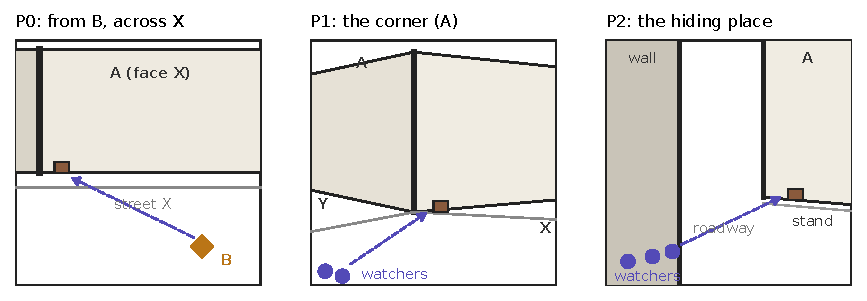
\includegraphics[width=0.92\textwidth]{figures/fig01_sketches.pdf}
\caption{The three views as diagrams (nothing is traced from the drawings). P0: from the licensed-establishment side across X, the clothes shop on the X face of corner A and the boy at its foot (ch.~0 p.~14 panel~4\textsuperscript{*}). P1: the inked corner from the watchers' side, across a roadway, both faces visible and the stand on the right-hand face (ch.~1 p.~7 panel~4). P2: the hiding view, with the family against a wall beside a quoined edge and the boy beyond it on the same frontage (ch.~1 p.~6 panel~6; p.~7 panel~6 and the pencil draft, p.~6 panel~8\textsuperscript{*}, agree). Unlike P1, P2 draws no street between them; the geometry follows P1, and P2 is not used as a constraint (Section~\ref{sec:result}). A: corner block; B: licensed establishment; X and Y: modelled streets.}\label{fig:sketches}
\end{figure}

\section{What the archives tell us}\label{sec:archives}
\paragraph{Sources.} The Ordnance Survey 1:500 town plan of Glasgow, sheets Lanarkshire VI.10.15 and VI.10.20, surveyed in 1857--58 and published in 1859, in the georeferenced layer of the National Library of Scotland \citep{nls1857}: the nearest large-scale survey before 1877, and it draws building lines, pends, closes and recesses. The 1:500 plan of 1892--94, to see what had changed \citep{nls1893}. The Post Office Annual Glasgow Directory, the 1877--78 volume for the year of the story and fourteen others from 1860--61 to 1905--06 to follow particular addresses \citep{pod}. The Canmore catalogue description and the directories for Paisley's \citep{canmorePaisley,gracesPaisley}. Ottens objects that Jamaica Street had a tramline from 1872, so that the street where the visitor arrives cannot be Jamaica Street \citep{ottens2020neverwas}; the first line of the Glasgow Tramway and Omnibus Company opened on 19 August 1872 and ran by way of Renfield Street and the Jamaica Bridge \citep{wikiGlasgowTram}, which stands at the foot of Jamaica Street. That summary does not name Jamaica Street itself, and tram service there in 1877 is not documented here. The present test does not model traffic or street furniture, so the objection is neither met nor refuted here. If the panels show no rails, which was not checked here, their absence would measure how literally Rosa drew 1877 rather than where he set the scene; read literally, it would count against the two corners of Table~\ref{tab:corners} whose watched street is Jamaica Street; tram service in 1877 was not checked for the streets watched at the other three. Gardner's Warehouse at 36 Jamaica Street (1855--56) still stands \citep{hesGardner}; it lies north of Ann Street, not on the frontage facing the candidate corner.

\paragraph{Problems of date.} The sources do not share a year with the story \citep{plewe2002uncertainty}. The best plan predates it by twenty years and the next follows it by fifteen, so a feature drawn in 1857 and gone by 1893 is unattested for 1877 itself. The sign is later than the story. In 1876--79 Peter Paisley is listed ``of S.S. Clothing Co.'' on the south bank; 72 Jamaica Street is Abraham Rowand's in the 1877--78 trades list and the 1878--79 street section, has no entry in the 1879--80 street sequence, and is Paisley's in the 1880--81 and 1881--82 volumes only. Later volumes place Paisley's at 80 and 96 Jamaica Street (1885--86), then at 82 to 96 Jamaica Street and 2--12 Broomielaw (1890--91), called the Broomielaw corner in 1895--96. The sign therefore points to a later phase of the same frontage, not to an address continuously occupied by Paisley's. Ottens reproduces an early twentieth-century view of Jamaica Street with Paisley's on the left, notes that the real storefront looked different from Rosa's and that Rosa's street lamps look like the real ones \citep{ottens2020neverwas}; on that photograph the author reads the fascia ``96 PAISLEY'S''. A view of that kind is one plausible route for the later sign, but whether such a view also shows the Howard Street corner has not been checked.

\paragraph{Procedure.} The implemented census has five reproducible steps:
\begin{enumerate}
\item Place the later Paisley's corner (Jamaica Street and the Broomielaw: 96 Jamaica Street from 1885--86, called the Broomielaw corner in 1895--96) on the 1857 plan and define a reproducible survey window from Argyle Street to the Clyde and from Oswald Street to St Enoch's Square (Figure~\ref{fig:situation}). This is not a strict radius: three recorded corners lie at approximately 205, 251 and 263~m from that point, while the two Broomielaw--Wood Lane corners at 55 and 66~m are outside the twelve selected facing facades.
\item Record every opening (covered pend, open recess, street mouth) on those twelve facades: \nOpenings\ openings. Each physical corner is enumerated with a street as Y only where one of the twelve facades faces the corner across that street; this gives \nCornersOriented\ orientations of \nPhysicalCorners\ physical corners (the reference file lists 26 points: the \nPhysicalCorners\ used and the two Wood Lane corners that no selected facade faces). Pairing each orientation with openings on its facing facade gives \nUniverse\ configurations. The claim is conditional on this declared window and facade selection.
\item Measure street widths facade to facade with the viewer's measuring tool, good to about $\pm0.7$~m. At the candidate corner, widths recomputed from the recorded corner coordinates differ from these by under 1~m; elsewhere the difference reaches about 2.5~m.
\item Apply the relations of H5 and the author's contested H7 filter to every configuration: the opening on the side of X ($d>0$, where $d$ is the offset of its nearer wall along the axis of Y, measured from the line through A perpendicular to Y, and $D$ the straight-line distance from that wall to the corner), X on the watchers' right, $1.5\le w_Y/w_X\le 3$, and the stand's face seen at $15$\degree\ or more, the angle being taken as $\arctan(d/w_Y)$. The model thus treats Y and X as perpendicular; Section~\ref{sec:result} also reports the census with visibility and angles measured on the plan. The distance threshold that the author's earlier working dossier attached to H8 is reported, but not applied to the principal model, in Section~\ref{sec:result}.
\item Read the 1877--78 directory for every corner that survives step 4: the trade at the corner premises and the licensed premises on the block facing the stand.
\end{enumerate}
The counts are \nUniverse\ $\to$ \nCone\ (both faces visible) $\to$ \nCtwo\ (X on the right) $\to$ \nCthree\ (width ratio) $\to$ \nAngle\ (viewing angle), on \nCorners\ corners. The geometry alone therefore does not single out a corner. What it does do is exclude the later Paisley's corner itself: the north-west corner of Jamaica Street and the Broomielaw enters the census with \nBroomielawNW\ configurations and fails the first relation, since every opening on the frontage facing it lies north of the Broomielaw mouth, so no watcher there sees both faces with the side street on the right.

\begin{figure}[htbp]\centering
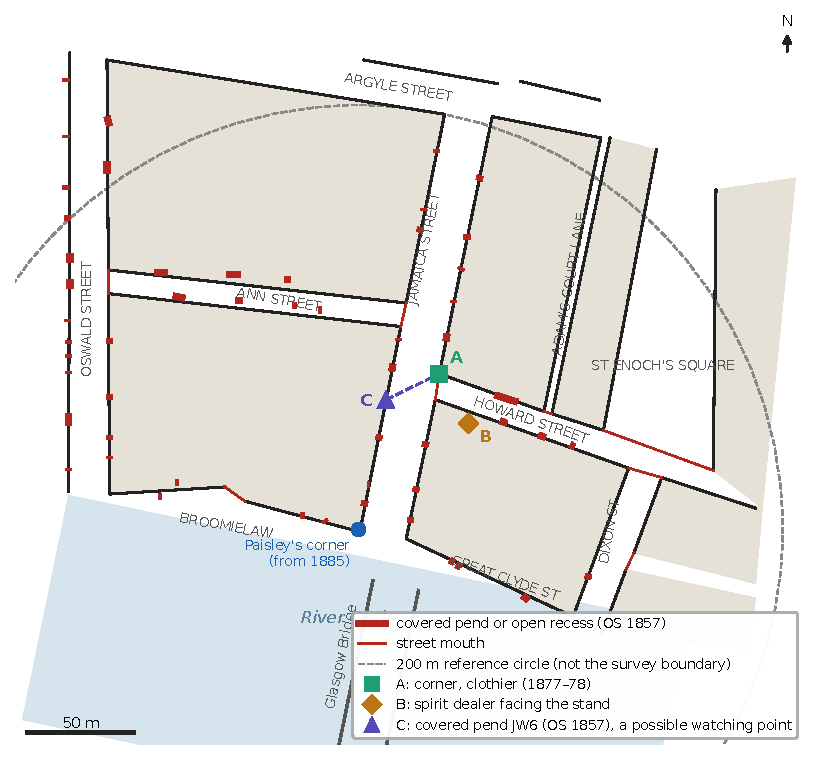
\includegraphics[width=0.52\textwidth]{figures/fig02_situation.pdf}
\caption{The survey window at the foot of Jamaica Street, redrawn, not reproduced as a facsimile, from the OS 1:500 plan surveyed 1857--58 \citep{nls1857} (National Library of Scotland georeferenced layer, re-use stated as CC-BY (NLS), consulted 9 November 2026). Red marks are the \nOpenings\ recorded openings. The blue point marks the later Paisley's corner at the Broomielaw; the 1880--82 address lay further north on the same frontage. A, B and C are the corner, the licensed premises and the pend of Section~\ref{sec:result}.}\label{fig:situation}
\end{figure}

\section{A corner in Glasgow}\label{sec:result}
\paragraph{The five corners.} Table~\ref{tab:corners} lists the \nCorners\ corners that pass the author's geometric model, with their nearest admissible opening and the 1877--78 evidence found for their trades. All \nRivals\ rivals offer a nearer opening or a wider viewing angle than the retained candidate, and in the model Jamaica Street and Ann Street is almost its geometric twin (\AnnSWD~m and \AnnSWAngle\degree, against \SfourD~m and \SfourAngle\degree; on the plan \AnnSWAnglePlan\degree\ against \SfourAnglePlan\degree); the geometry favours none of the five. Only the north-east corner of Jamaica Street and Howard Street has both a verified clothier at the corner and verified licensed premises facing the stand across the narrow street. All the rival evidence comes from the OCR (optical character recognition) text of the scanned directory. Two rivals have affirmative evidence of other trades at the corner; for the other two the occupants found could not be tied to the corner premises (Dixon Street and Fox Street) or the OCR does not mark where Ann Street crosses the Oswald Street sequence (Ann Street and Oswald Street), so their trades remain unknown and are not treated as negative evidence.

\begin{table}[htbp]\centering\scriptsize
\caption{The corners that pass the author's geometric filters, ordered by the distance $D$ from the corner to the nearest admissible opening, with the 1877--78 directory evidence \citep{pod}. ``Partial'' is an imperfect positional or trade match; ``no'' is used where the 1877--78 directory gives the corner premises to a named non-clothier; ``unknown'' where the occupants found could not be tied to the corner premises, or where the OCR text was silent, since absence from OCR is not evidence of absence. Generated from the data by the companion code.}\label{tab:corners}
\begin{tabular}{>{\raggedright\arraybackslash}p{2.7cm}>{\raggedright\arraybackslash}p{1.8cm}rr>{\raggedright\arraybackslash}p{3.9cm}>{\raggedright\arraybackslash}p{3.8cm}}
\toprule
Corner A (Y / X) & Nearest opening & $D$ (m) & Angle & At the corner, 1877--78 & Facing the stand across X, 1877--78 \\
\midrule
Howard $\times$ Adam's Court Lane NW (Howard / ACL) & HS3, covered pend (2 admissible) & 20.0 & 56$^\circ$ & Corson \& Currie, fish, ice and oyster merchants: clothier no & M'Laughlin, Patrick, wine and spirit merchant: licensed partial \\
Dixon $\times$ Fox NE (Dixon / Fox) & DW1, covered pend (1 admissible) & 23.5 & 46$^\circ$ & Calder Ironworks office. Metzenburgh \& Co., furriers and skin merchants: clothier unknown & not found in OCR: licensed unknown \\
Jamaica $\times$ Ann SW (Jamaica / Ann) & JE4, covered pend (4 admissible) & 27.3 & 35$^\circ$ & Dryburgh, William, wine and spirit merchant: clothier no & Blair, Campbell, tea and wine merchant and grocer: licensed partial \\
\textbf{Jamaica $\times$ Howard NE} (Jamaica / Howard) & JW6, covered pend (4 admissible) & 27.8 & 37$^\circ$ & Morrison, Hugh, clothier and Highland costume maker: clothier yes & Turner, J. B., spirit dealer: licensed yes \\
Ann $\times$ Oswald NE (Oswald / Ann) & OW7, covered pend (6 admissible) & 30.3 & 50$^\circ$ & not identified: the OCR of the even side (22 Wilson, ship stores, 24-26 Sinclair, Moorhead, produce merchants, 28-32 Stewart \& Co.) does not mark where Ann St crosses: clothier unknown & not identified: a wine merchant at 38 and a spirit dealer at 42 on the even side, position relative to Ann St not marked: licensed unknown \\
\bottomrule
\end{tabular}

\end{table}

\paragraph{Geometry.} The north-east building corner is approximately \DPaisleyA~m in plan distance from the later Paisley's corner at the Broomielaw. The 1880--82 address, 72 Jamaica Street, lay on the same west frontage between Colosseum Buildings (68) and that corner, since numbers 74 and 76 were still in use in 1879--80; the plan carries no numbers, so it is not placed more precisely. Jamaica Street is measured as $\WidthJamaica\pm0.7$~m wide and Howard Street as $\WidthHoward\pm0.7$~m, a central ratio of~\RatioJH. Place the stand on the Howard Street face of the corner. For a watcher on the west side of Jamaica Street looking at that corner, Howard Street leaves on the right. On that west side, \Sfourd~m south of the corner measured along Jamaica Street, the 1857 plan draws a covered passage 2.8~m wide (\SfourOpen) leading to a small court, plausibly associated by address alone with ``Smith's Court, 62 Jamaica street'' in the directory index. The plan carries no street numbers: number 62 is placed by counting from 68, Colosseum Buildings, whose number is given in 1860--61 and 1881--82 and appears stable in the sampled volumes, and the association rests on that count alone. From its north wall a watcher would see both the Jamaica Street front and the Howard Street return of the corner block, the stand's face at \SfourAngle\degree\ in the model and \SfourAnglePlan\degree\ on the plan, where the two faces of the corner meet at about \CornerAngleJH\degree, \SfourD~m from the corner edge (Figure~\ref{fig:corner}). The filters admit \nSfourAdmissible\ openings for this corner, JW6--JW9; JW6 is the nearest and is reported.

\paragraph{Trades.} ``53 Morrison, Hugh, clothier'' is the last entry on the east side of Jamaica Street before ``Howard street intersects'' (p.~575); his full entry reads ``clothier and Highland costume maker, 51 and 53 Jamaica street, and 1, 3, 5, 9 Howard st.'' (p.~351), so Morrison's listed addresses wrap the corner. In Howard Street, ``6 Turner, J.~B. spirit dealer'' (p.~573) is on the south block facing the stand. If the ``P.H.'' (public house) marked on the 1892--94 plan is the same premises, it lies about 18~m east along Howard Street from the south-east building corner at Jamaica Street; the identification is not proved. The sampled volumes list a clothier at 53 Jamaica Street in 1860--61, 1865--66, 1870--71 and in every sampled year from 1876--77 to 1895--96 (Hugh Morrison to 1891--92, R.~W. Forsyth from 1892--93); the 1905--06 line names Forsyth without a trade. They list a spirit dealer at 6 Howard Street in every sampled year from 1860--61 to 1895--96; the 1905--06 line gives Turner's company and address without a trade.

\begin{figure}[htbp]\centering
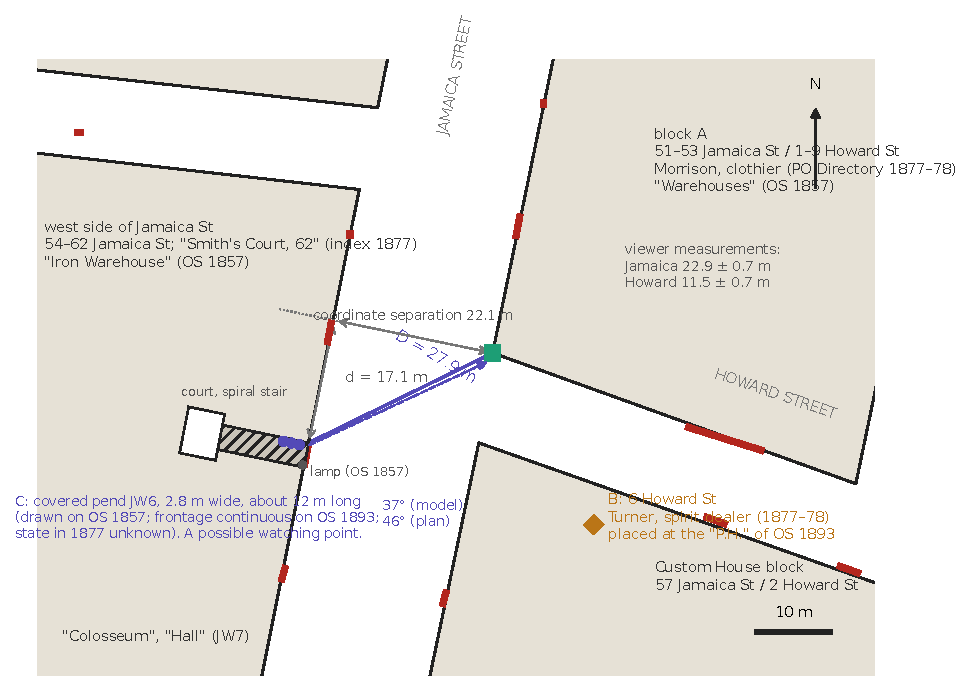
\includegraphics[width=0.6\textwidth]{figures/fig03_corner.pdf}
\caption{Jamaica Street and Howard Street at plan scale, redrawn, not reproduced as a facsimile, from the OS survey of 1857--58 \citep{nls1857}; National Library of Scotland georeferenced layer, CC-BY (NLS). A: north-east corner, Hugh Morrison, clothier, 1877--78. B: 6 Howard Street, J.~B. Turner, spirit dealer, 1877--78, tentatively placed at the ``P.H.'' of the 1892--94 plan. C: covered passage \SfourOpen, drawn in 1857, a possible watching point from which both faces of A are visible; the angle at C is given as the census computes it, treating the streets as perpendicular, and as measured on the plan. $d$, $D$ and the plotted positions are derived from the same coordinate data; the separately measured street widths are rounded and carry $\pm0.7$~m uncertainty. Approximate coordinates: A 55.8572, $-$4.2571; C 55.8571, $-$4.2575.}\label{fig:corner}
\end{figure}

\paragraph{What the proportions say.} A drawn page is not a survey: to keep the watchers, the boy and the shop in one frame, the cartoonist shortens depth and widens what must be read \citep{lefevre2008space}. The drawn proportions are therefore reported as a test of the model, not of the corner. The author's earlier working dossier, which is not deposited, recorded before the census a rule: if the watchers were drawn clearly nearer than twelve adult heights (\CfiveWorking~m), the window would offer no configuration that reproduces the drawing. The rule is reported, not applied; its date rests on that undeposited dossier. The central model readings put the watchers at 3.5 to 5 heights, with every upper bound at or below ten (\CfiveEnvelope~m); the author's reading is four to six. The nearest admissible opening under the principal filters is \DminAll~m from its corner and \SfourOpen\ is \SfourD~m, \SfourH\ adult heights away. None of the \nAngle\ principal survivors remains at $D\le\CfiveEnvelope$~m; \nCfiveWorking\ remains at $D\le\CfiveWorking$~m, opening HS3 at Howard Street and Adam's Court Lane NW, rather than at the candidate (on the plan, \nCfiveWorkingPlan, with opening OW6 at Ann Street and Oswald Street NE at \DminPlan~m). Every reading of the drawn distance, the author's four to six heights as well as the models' envelope, is shorter than the nearest admissible opening, as the rule anticipated; that is what one expects of a page that compresses a street to the width of a panel. The drawn distance does not discriminate between candidates and is not used as a filter. The width ratio is different: 1.5--3 remains an explicit, contested author-defined filter on which the five-corner comparison is conditional. Replacing it with the model-read interval 0.4--1.6 removes Jamaica and Howard (\RatioJH) and leaves \nModelRatio\ configurations on \nModelCorners\ corner, Howard Street and Dixon Street SE, whose corner premises the 1877--78 directory gives to a non-clothier (a restaurant, if the even numbers of Dixon Street lay on its east side), so that no corner surviving that reading has both trades. The distance test uses the envelope of the model readings (up to ten heights), whereas 0.4--1.6 is the range of their central values; applied in the same way to the ratio, their envelope (0.2--4.0) keeps Jamaica and Howard and gives \nModelEnvelope\ configurations on \nModelEnvelopeCorners\ corners. Removing the ratio altogether gives \nNoRatio\ configurations on \nNoRatioCorners\ corners and adds Howard Street and Dixon Street SE and Howard Street and St Enoch's Square NW; neither has a clothier at the corner premises in 1877--78 (a fruiterer at the latter, with clothiers listed nearby at 27 Howard Street and 52 St Enoch's Square), and licensed premises facing the stand were not found in the OCR text at either. The test therefore rests on the drawn relations and on the declared filters, not on the drawn proportions.

\paragraph{Two views of the watchers.} The inked pages stage the watchers twice. In ch.~1 p.~7 panel~4 they look at the corner across a roadway, both faces in view. In p.~6 panel~6 and p.~7 panel~6 they stand against a brick wall beside a quoined edge, with no street drawn between them and the boy, who is beyond the edge on the same frontage (the pencil draft agrees). The two cannot be combined on one plan. The geometry follows p.~7 panel~4, the only view that shows both faces of the corner and the street between; the hiding views frame the family, not the street layout, and are not used as constraints. H6 still fixes the kind of watching point: the census looks for openings in the facing frontage, so a pend such as JW6 is a possible watching point, not the hiding place drawn, and the plan offers a covered pend where the hiding views draw a building edge.

\paragraph{Sensitivity.} Table~\ref{tab:sens} varies the author's thresholds and the contested readings. The candidate survives the stated width uncertainty, removal of the handedness convention, the envelope of the model-read ratios and the plan angles, but not the range of the central model ratios or either distance threshold. The model treats the two streets of each corner as perpendicular; measured on the plan, against the recorded face X, visibility and viewing angle give \nPlanAngle\ configurations on the same \nPlanCorners\ corners, the candidate being seen at \SfourAnglePlan\degree\ rather than \SfourAngle\degree, while opening OW6 at Ann Street and Oswald Street NE enters at \DminPlan~m. Removing handedness gives \nNoHand\ configurations on \nNoHandCorners\ corners; this is not a documentary uniqueness test because the newcomers were not all checked.

\begin{table}[htbp]\centering\footnotesize
\caption{Survivors of the geometric step under other settings (generated by the companion code). The documentary step is applied in full to the five corners of the published setting; the two corners that enter only under the width-ratio variants were read in the OCR text only, and the other corners that enter under other settings were not checked. The rows on the model-read ratios and on distance test the drawn proportions; they are reported, not applied.}\label{tab:sens}
\begin{tabular}{>{\raggedright\arraybackslash}p{7cm}rrl}
\toprule
Geometric setting & Corners & With both trades & Jamaica $\times$ Howard NE kept \\
\midrule
every frontage point, handedness kept & 8 & 1 & yes \\
every frontage point, no handedness & 14 & 2 & yes \\
first coding: lanes kept, clothier anywhere at the corner & 10 & 2 & yes \\
first coding, no handedness & 17 & 3 & yes \\
1857 openings only, first coding (version 1.4 without its width-ratio filter) & 7 & 1 & yes \\
1857 openings only, width ratio 1.5--3, first coding (version 1.4 as published) & 5 & 1 & yes \\
1857 openings only, no handedness & 10 & 1 & yes \\
width ratio 1.5--3 (used up to version 1.4) & 4 & 1 & yes \\
angle $\ge 10^\circ$ & 9 & 1 & yes \\
angle $\ge 25^\circ$ & 8 & 1 & yes \\
widths: $Y$ $+0.7$~m, $X$ $-0.7$~m & 8 & 1 & yes \\
widths: $Y$ $-0.7$~m, $X$ $+0.7$~m & 8 & 1 & yes \\
visibility and angle measured on the plan & 9 & 1 & yes \\
distance $D \le 20.4$~m (author's earlier rule) & 4 & 0 & no \\
\bottomrule
\end{tabular}

\end{table}

\paragraph{Alternatives.} Three remain open. Reversing the orientation, with the stand on the Jamaica Street face and the watchers across Howard Street, is not a single-criterion alternative: the width ratio becomes about \RatioMirror, outside the author's band though inside the model-read one, none of the four openings on the south side of Howard Street (three pends and the mouth of Dixon Street) sees both faces of the corner, and Jamaica Street would leave on the watchers' left. A composite set remains possible because the sign and corner are not shown in one frame, the watchers are staged in two incompatible ways, the corner panel is marked as a rerun and Rosa recreated panels from the 1963 and 1964 stories \citep{ottens2020clan}; nothing here refutes that construction. Finally, the documentary test is comparative, not probabilistic: the two verified trades discriminate among the five corners produced by the declared filters, not among all of Glasgow's corners. Nor is a clothier a rare find on this street: Ottens calls Jamaica Street the centre of Glasgow's drapery trade \citep{ottens2020neverwas}, and the 1877--78 lines in Appendix~\ref{app:directories} name clothiers at 61, 65 and 72 Jamaica Street and costumiers at 1--7. A clothier at a Jamaica Street corner is therefore weak evidence on its own; the weight lies in its conjunction with licensed premises across the narrow street, within the five corners that the geometry admits.

\begin{table}[htbp]\centering\small
\caption{What each source attests. ``Measured'' is read from the georeferenced plan; ``inferred'' joins several observations.}\label{tab:evidence}
\begin{tabular}{>{\raggedright\arraybackslash}p{2.9cm}>{\raggedright\arraybackslash}p{4.0cm}>{\raggedright\arraybackslash}p{5.2cm}>{\raggedright\arraybackslash}p{2.5cm}}
\toprule
Feature & Source & Finding & Status \\
\midrule
Street (H2) & Directories; Canmore catalogue & Paisley's at 72 Jamaica Street in 1880--81 and 1881--82 & attested, 1880--82 \\
Street geometry & OS 1:500, surveyed 1857--58 & \WidthJamaica~m and \WidthHoward~m; X on the watchers' right; faces meeting at about \CornerAngleJH\degree & measured \\
Corner trade & Directory 1877--78, pp.~351, 575 & Hugh Morrison, clothier & attested \\
Facing trade & Directory 1877--78, p.~573 & J.~B. Turner, spirit dealer & attested \\
Watching point (P1) & OS 1857; index 1877--78; panels & 2.8~m covered passage, \SfourD~m from the corner; ``Smith's Court, 62''. The hiding views draw a building edge on the boy's own frontage and cannot be placed on the plan & drawn 1857; 1877 unknown \\
Drawn distance (H8) & panels; model readings & 4--6 adult heights against \SfourH & not met; compressed, as drawn pages are \\
Width ratio (H7) & panels; model readings & \RatioJH\ against 0.4--1.6 (envelope 0.2--4.0) & contested \\
Location of scene & all of the above & Jamaica Street and Howard Street, north-east corner & probable identification \\
\bottomrule
\end{tabular}
\end{table}

\section{A dime, a street corner, and the strongest match}\label{sec:conclusion}
Within the \nUniverse\ configurations on the twelve selected facades, the author's ratio band and the other declared filters produce five corners. Among those five, the north-east corner of Jamaica Street and Howard Street is the only one with affirmative 1877--78 evidence for both a clothier at the corner and licensed premises across the side street. It also has the required handedness, a view of both faces from the opposite frontage, as the inked corner view (ch.~1 p.~7 panel~4) shows, and \nSfourAdmissible\ admissible openings there. Two rivals have a non-clothier at the corner and only a partial match for the bar, and two remain incompletely checked; none of the other four has both trades attested.

The proportions are a weaker witness. No reading of the drawn distance is met by any of the five corners, and the range of the model-read central width ratios removes Jamaica and Howard, though their envelope keeps it; but a comics page compresses depth to serve the story, the model intervals are broad, and no panel measures both streets cleanly. Those proportions justify caution about a literal reconstruction, but they do not outweigh the named street, the corner geometry and the paired 1877--78 trades. A composite set remains possible because the sign and the corner do not share a frame, the watchers are staged in two incompatible ways and the corner panel is marked as a rerun, but possibility alone does not put it on equal footing with the documented match.

Our confidence is therefore graduated. We have high confidence that Jamaica and Howard NE is the strongest candidate in the declared survey window, and we judge it probable that this corner supplied the topographic basis of the shoeshine scene. Confidence is lower that Rosa copied one single real view rather than combining references or compressing the streets. Evidence of Rosa's source images, such as period views of Jamaica Street, a dated view establishing whether the opening at number 62 existed in 1877, or an independent human reading that reverses the side street would materially change that assessment. We could not read the 1877--78 valuation roll for 6 Howard Street \citep{nrsVR102,spVR} or verify the passage in a source dated to 1877. On the evidence now available, and within the declared window and filters, the most likely place where Scrooge earned his dime is the north-east corner of Jamaica Street and Howard Street.

\section*{Data and code availability}
Survey files, the directory extracts for the five corners and for the two corners that enter under the width-ratio variants, census code (including the sensitivity variants), generated tables and figure scripts are in \repourl. The command \texttt{make all} regenerates tables, figures and paper; \texttt{make test} checks the counts, measurements and sensitivities, including the distance thresholds at 17~m and 20.4~m and the plan angles. The author's photographs of directory pages and of the comic pages are not distributed.

\section*{Generative AI use statement}
\href{https://claude.ai}{Claude} (Anthropic) and \href{https://chatgpt.com}{ChatGPT}/\href{https://openai.com/codex/}{Codex} (OpenAI), accessed in November 2026, were used for OCR assistance, language revision and code review, including revisions to deterministic plotting scripts. Five exploratory model readings supplied the distance and width-ratio intervals and the handedness reading used in the sensitivity analysis; they are not independent human observations. The author's 1.5--3 width-ratio band (H7) was adopted from a single earlier exploratory reading by ChatGPT. The release contains a concise aggregate record of that protocol and its numerical results (\texttt{evidence/model\_reading\_sensitivity.md}), not raw prompts or conversations. No model output is treated as archival evidence. The human author checked the quoted directory lines against the OCR text, and on the page images where marked $\dagger$ in Appendix~\ref{app:directories}, checked the cited sources, ran the code, reviewed every figure and accepts responsibility for the analysis and text.

\section*{Licences}
Original text, tables, diagrams and the data files are licensed CC BY 4.0. Source code is licensed MIT. Third-party map information retains its stated attribution and reuse conditions; the directory lines are transcribed from the National Library of Scotland digitisation on the Internet Archive, published under CC BY-NC-SA 2.5 Scotland. No comic panel, page, scan or tracing is distributed.

\section*{Acknowledgements}
Figures~\ref{fig:situation} and \ref{fig:corner} are redrawn from the Ordnance Survey town plans in the georeferenced layers of the National Library of Scotland, under the Library's stated CC-BY (NLS) re-use terms.

\bibliographystyle{plainnat}
\bibliography{refs}

\appendix
\section{Directory lines relied on}\label{app:directories}
\scriptsize
Post Office Annual Glasgow Directory \citep{pod}; lines marked $\dagger$ were checked on the page image by the author, the others in the OCR text.

\textbf{1877--78.} General section, p.~351: ``Morrison, Hugh, clothier and Highland costume maker, 51 and 53 Jamaica street, and 1, 3, 5, 9 Howard st.''$^\dagger$ Street section, Jamaica Street, east side, p.~575: ``53 Morrison, Hugh, clothier'' immediately precedes ``Howard street intersects''$^\dagger$; then ``57, 59 Gordon, Robt.'' (umbrella and portmanteau manufacturer), ``61 Buchanan \& Johnson, clothrs.'', ``65 Adamson, A. \& W. clothiers''. Howard Street, p.~573: ``8, 10, 12, Westlands, Laidlaw, \& Co. hat \& cap manufs. / 6 Turner, J.~B. spirit dealer / 2 Falconer, \& Co.''$^\dagger$; trades list: ``Turner, J.~B. 6 W. Howard st. and 20 Lancefield street'' (the same entry as ``6 Turner'' in the Howard Street section). Jamaica Street, west side: ``Rowand, A. clothier''$^\dagger$, listed at 72 (and once at 70) in the trades lists. Street index, p.~69: ``Smith's Court, 62 Jamaica street. 7.'' General section, p.~370: ``Paisley, Peter (of S.S. Clothing Co.), 373 Govan st.'' Rival corners: ``11, 15 Corson \& Currie'' (fish, ice and oyster merchants); ``M'Laughlin, Patrick, wine and spirit merchant, 21 Howard street''; ``Dryburgh, William, wine and spirit merchant, 44 Jamaica street'' (street section, p.~576: ``44 Dryburgh, W. spirit mer. / Ann street intersects''); ``Blair, Campbell, wholesale and retail tea and wine merchant and grocer, 38, 40 Jamaica street''; ``Calder Ironworks office, 1 Dixon street''; ``2, 6 Metzenburgh \& Co.'' (Fox Street; furriers and skin merchants); Oswald Street, p.~600: ``22 Wilson, J. \& R. ship stores'', ``24, 26 Sinclair, Moorhead, \& Co.'', ``28, 30, 32 Stewart, John, \& Co.'', ``38 Taylor \& Ferguson, wine mer.'', ``42 Kirkham, Thos. spirit dealer'', the OCR not marking where Ann Street crosses the sequence. Other Jamaica Street entries: ``1, 3, 5, 7 Simpson, R. \& Sons'' (costumiers, silk mercers; Argyle Street corner); ``11 Paxton, Matthew, spirit mer.'' Corners entering only under sensitivity settings: Alexander Conacher, proprietor of the Lorne Restaurant (``Lome'' in the OCR), 22 Dixon street and 40 Howard street; ``Adam, James, fruiterer, 58 St. Enoch square and 29, 31 Howard st.''; the side of Dixon Street on which 22 lay is inferred from the numbering, and the OCR lines are in \texttt{data/directory\_lines.md}.

\textbf{Other years} (fourteen sampled volumes besides 1877--78, from 1860--61 to 1905--06) are transcribed in \texttt{data/directory\_lines.md}. The 1870--71 general section, p.~274, gives ``Morrison, Hugh, naval \& military clothier, Highland costume maker, and gentlemen's complete outfitter, 51 and 53 Jamaica street and 1, 3, 5, 9 Howard street''; the 1905--06 line for 4--6 West Howard Street gives the company and address but not its trade.\par
\normalsize

\end{document}
